\documentclass{llncs}

\usepackage{graphicx}

\begin{document}

\begin{abstract}
A fixed bit-width counter was proposed as a proof-of-concept demonstration of an oritatami model of cotranscriptional folding [Geary et al., Proc.~MFCS 2016, LIPIcs 58, 43:1-43:14], and it was embedded into another oritatami system that self-assembles a finite portion of Heighway dragon fractal. 
In order to expand its applications, we endow this counter with capability to widen bit-width at every encounter with overflow. 
\end{abstract}

\section{Introduction}

Counting is one of the most essential tasks for computing; as well known, it suffices to count for Turing universality \cite{Minsky1967}. 
Nature has been counting billions of days using molecular ``circadian clockwork'' which is ``as complicated and as beautiful as the wonderful chronometers developed in the 18th century''  \cite{McClung2006}. 
Nowadays, developments in molecular self-assembly technology enable us to design molecules to count. 
Evans has recently demonstrated a DNA tile self-assembly system that counts accurately in binary from a programmed initial count until it overflows \cite{EvansPhD}. 
In its foundational theory of molecular self-assembly, such binary counters have proved their versatility, being used to assemble shapes of particular size \cite{AdChGoHu2001,RothemundWinfree2000}, towards self-assembly of fractals \cite{MasudaSekiUbukata2018}, as an infinite scaffold to simulate all Turing machines in parallel in order to prove undecidability of nondeterminism in the abstract tile-assembly model \cite{BrChDoKaSe2013}, and so on. 

\begin{figure}[tb]
\centering
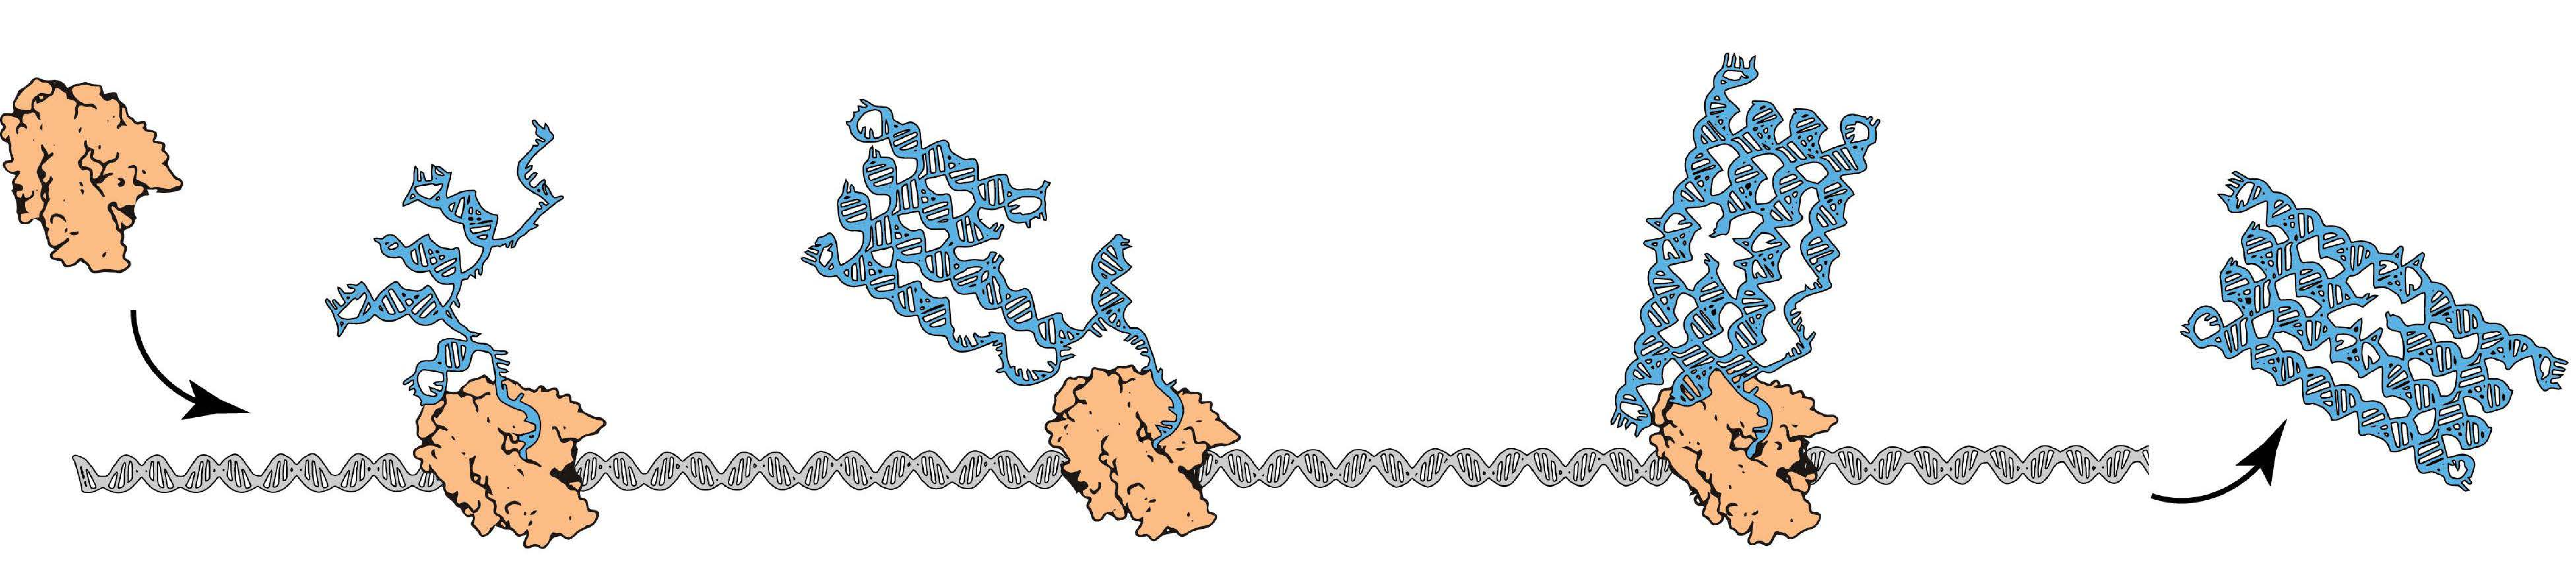
\includegraphics[width=\linewidth]{rna_origami.pdf}
\caption{RNA origami}
\label{fig:rna_origami}
\end{figure}

A fixed bit-width (finite) binary counter has been implemented as a proof-of-concept demonstration of oritatami model of cotranscriptional folding \cite{GeMeScSe2019}. 
As shown in Fig.~\ref{fig:rna_origami}, an RNA transcript folds upon itself while being transcribed (synthesized) from its corresponding DNA template strand. 
Geary et al. programmed a specific RNA rectangular tile structure into a DNA template in such a way that the corresponding RNA transcript \textit{folds cotranscriptionally} into the programmed tile structure highly likely \textit{in vitro} at room temperatures (\textit{RNA origami}) \cite{GearyRothemundAndersen2014}. 
An oritatami system folds a transcript of abstract molecules called \textit{beads} of finitely many types cotranscriptionally over the 2-dimensional triangular lattice cotranscriptionally according to a rule set that specifies which types of molecules are allowed to bind. 
The transcript of the binary counter in \cite{GeMeScSe2019} is of period 60 as $\textcircled{\scriptsize 0}{-}\textcircled{\scriptsize 1}{-}\textcircled{\scriptsize 2}{-} \cdots {-}\textcircled{\scriptsize 58}{-}\textcircled{\scriptsize 59}{-}\textcircled{\scriptsize 0}{-}\textcircled{\scriptsize 1} \cdots$ and its period is semantically divided into two half-adder (HA) modules $A = \textcircled{\scriptsize 0}{-}\textcircled{\scriptsize 1}{-} \cdots {-}\textcircled{\scriptsize 11}$ and $C = \textcircled{\scriptsize 30}{-}\textcircled{\scriptsize 31}{-} \cdots {-}\textcircled{\scriptsize 41}$ and two structural modules $B$ and $D$, which are sandwiched by half-adder modules.
While being folded cotranscriptionally in zigzags, HA modules increment the current count $i$ by 1, which is initialized on a linear \textit{seed} structure, alike the Evans' counter, whereas structural modules $B$ and $D$ align HA modules properly and also make a turn at an end of the count $i$; $B$ guides the transcript from a zig to a zag ($\hookrightarrow$) while $D$ does from a zag to a zig ($\hookleftarrow$). 
This counter was embedded as a component of an oritatami system to self-assemble an arbitrary finite portion of Heighway dragon fractal \cite{MasudaSekiUbukata2018}. 
Its applications is limited, however, by lack of mechanism to widen bit-width; its behavior is undefined when its count overflows. 
In this paper, we endow this counter, or more precisely, its structural module $B$, with capability to widen the count by 1 bit at every encounter with overflow. 

\begin{thebibliography}{1}

\bibitem{AdChGoHu2001}
Leonard Adleman, Qi Chang, Ashish Goel, and Ming-Deh Huang, 
Running time and program size for self-assembled squares, 
In Proc. STOC 2001, ACM, 740-748, 2001. 

\bibitem{BrChDoKaSe2013}
Nathaniel Bryans, Ehsan Chiniforooshan, David Doty, Lila Kari, and Shinnosuke Seki, 
The power of nondeterminism in self-assembly, 
\textit{Theory of Computing}, vol. 9, 1-29, 2013.

\bibitem{EvansPhD}
Constantine Glen Evans, 
Crystals that Count! Physical Principles and Experimental Investigations of {DNA} Tile Self-Assembly, 
Ph.D. thesis, Caltech, 2014.

\bibitem{GeMeScSe2019}
Cody Geary, Pierre-\'{E}tienne Meunier, Nicolas Schabanel, and Shinnosuke Seki, 
Oritatami: A computational model for molecular co-transcriptional folding, 
\textit{International Journal of Molecular Sciences} vol. 20(9), 2259, 2019. Its conference version was published in Proc. MFCS 2016. 

\bibitem{GearyRothemundAndersen2014}
Cody Geary, Paul W. K. Rothemund, and Ebbe S. Andersen, 
A single-stranded architecture for cotranscriptional folding of {RNA} nanostructures, 
\textit{Science} vol 345(6198), 799-804, 2014.

\bibitem{MasudaSekiUbukata2018}
Yusei Masuda, Shinnosuke Seki, and Yuki Ubukata, 
Towards the algorithmic molecular self-assembly of fractals by cotranscriptional folding, 
In Proc. CIAA 2018, LNCS 10977, Springer, 261-273, 2018.

\bibitem{McClung2006} 
C. Robertson McClung, 
Plant circadian rhythms, 
\textit{The Plant Cell}, vol. 18, 792-803, 2006.

\bibitem{Minsky1967}
Marvin Minsky, 
Computation: Finite and Infinite Machines, 
Prentice-Hall, Inc., 1967. 

\bibitem{RothemundWinfree2000}
Paul W. K. Rothemund and Erik Winfree, 
The program-size complexity of self-assembled squares (extended abstract), 
In Proc. STOC 2000, ACM, 459-468, 2000.

\bibitem{WinfreePhD}
Erik Winfree, 
Algorithmic Self-Assembly of {DNA}, 
Ph.D. thesis, Caltech, 1998.

\end{thebibliography}

\end{document}
